\documentclass[journal=jacsat,manuscript=article]{achemso}
\usepackage[utf8]{inputenc}
\usepackage[T1]{fontenc}       % Use modern font encodings
\usepackage{amssymb}
\usepackage[version=3]{mhchem} % Formula subscripts using \ce{}
\usepackage{siunitx}
\usepackage[table]{xcolor}

\usepackage{zref-xr,xc}
\usepackage{hyperref}
\zexternaldocument[M-]{ion_pairing_paper}
\externalcitedocument{ion_pairing_paper}

% Hack for making figures Say \figurename S\thefigure, e.g. Figure S1:
\makeatletter
\makeatletter \renewcommand{\fnum@figure}
{\textbf{Figure~S\thefigure}}
\makeatother

\renewcommand{\thetable}{\arabic{table}}
\makeatletter
\makeatletter \renewcommand{\fnum@table}
{\textbf{Tab.~S\thetable}}
\makeatother



\author{Hassan Srour}
\author{Martien Duvall Deffo Ayagou}
\author{Thi Thanh-Tam Nguyen}
\affiliation[Laboratoire de Chimie de l'ENS de Lyon]{Univ Lyon, Ens de Lyon, Univ Claude Bernard, CNRS,
Laboratoire de Chimie, F-69342 Lyon, France.}

\author{Nicolas Taberlet}
\author{Sébastien Manneville}
\affiliation[Laboratoire de Physique de l'ENS de Lyon]{Univ Lyon, Ens de Lyon, Univ Claude Bernard, CNRS,
Laboratoire de Physique, F-69342 Lyon, France.}


\author{Chantal Andraud}
\author{Cyrille Monnereau}
\affiliation[Laboratoire de Chimie de l'ENS de Lyon]{Univ Lyon, Ens de Lyon, Univ Claude Bernard, CNRS,
Laboratoire de Chimie, F-69342 Lyon, France.}

\author{Mathieu Leocmach}
\affiliation[Institut Lumière Matière]{Institut Lumière Matière, CNRS UMR 5306, Université Claude Bernard Lyon 1, Université de Lyon, Lyon, 69622 Villeurbanne Cedex, France}
\email{mathieu.leocmach@univ-lyon1.fr}


\title{Supplementary Informations to\\ Ion pairing controls rheological properties of ``processionary'' polyelectrolyte hydrogels}


\keywords{ATRP, hydrogel, poly(cations), rheology}

\begin{document}

%\section{Materials and methods}
All reactions were performed under an argon atmosphere using schlenk techniques. \ce{CH2Cl2} and THF were dried and degassed on a solvent station by passage through an activated alumina column followed by argon flush. All other solvents were used without additional purification. HEA purchased from Alfa Aesar was purified as reported in Ref~\cite{Srour2014} of the main text. Additional chemicals were obtained from Sigma Aldrich, Acros or Alfa Aesar and underwent no further purification. 

SEC analyses were carried out on ca \SI{5}{\milli\gram\per\milli\litre} solutions of each polymer in DMSO LiBr (\SI{0.01}{M}), using a MALVERN VISCOTEK 430  system equipped with three PSS Gram columns (Polyester Copolymer Network) set in series at \SI{80}{\celsius}, coupled to a Viscotek HT-GPC Module 350 A (refractive and viscosimeter) detector (at \SI{80}{\celsius}). The dispersity (\DJ = Mw/Mn) of the samples were derived from the RI signal by a universal calibration curve by pullulan. The number-average molar masses (Mn) were calculated from RI signals with the OmniSEC 4.6 software.

The thermal analysis was obtained on Differential Scanning Calorimetry (DSC). All samples were investigated using a Setaram DSC 131 apparatus. A weighed sample of \SI{5.0\pm 1}{\milli\gram} was placed in a sealed stainless crucible. A standard heating rate of \SI{5}{\kelvin\per\minute} was applied from 25 up to \SI{200}{\celsius} under \SI{50}{\milli\litre\per\minute} of nitrogen. The start and the onset temperatures were determined in order to assess the thermal stability. $T_\mathrm{start}$ is the temperature at which the sample starts to lose some mass and $T_\mathrm{onset}$ was determined from the step tangent method.

The high resolution mass spectra (MS QTOF) were recorded in positive and negative ion modes on a hybrid quadrupole time-of-flight mass spectrometer (MicroTOFQ-II, Bruker Daltonics, Bremen) with an electrospray ionization (ESI) ion source. The gas flow of the spray gas is \SI{0.6}{\bar} and the capillary voltage is $\pm\SI{4.5}{\kilo\volt}$. The solutions are infused at \SI{180}{\micro\litre\per\hour}. The mass range of the analysis is 50-1000~m/z and the calibration was done with sodium formate.

Frequency sweeps were performed within the linear domain by decreasing the frequency from $f=\SI{10}{\hertz}$ down to $f=\SI{0.01}{\hertz}$ at a strain amplitude $\gamma = 0.1 \%$ and at a temperature (\SI{25}{\celsius}) fixed by a Peltier plate. Strain sweeps were performed by ramping up the strain amplitude from $\gamma = 0.1 \%$ up to $\gamma =5000\%$ at $f=\SI{1}{\hertz}$ in the same temperature conditions. Most tests had to be stopped before the strain could reach its highest value due to sample ejection from the cone-plate geometry.

\begin{figure}
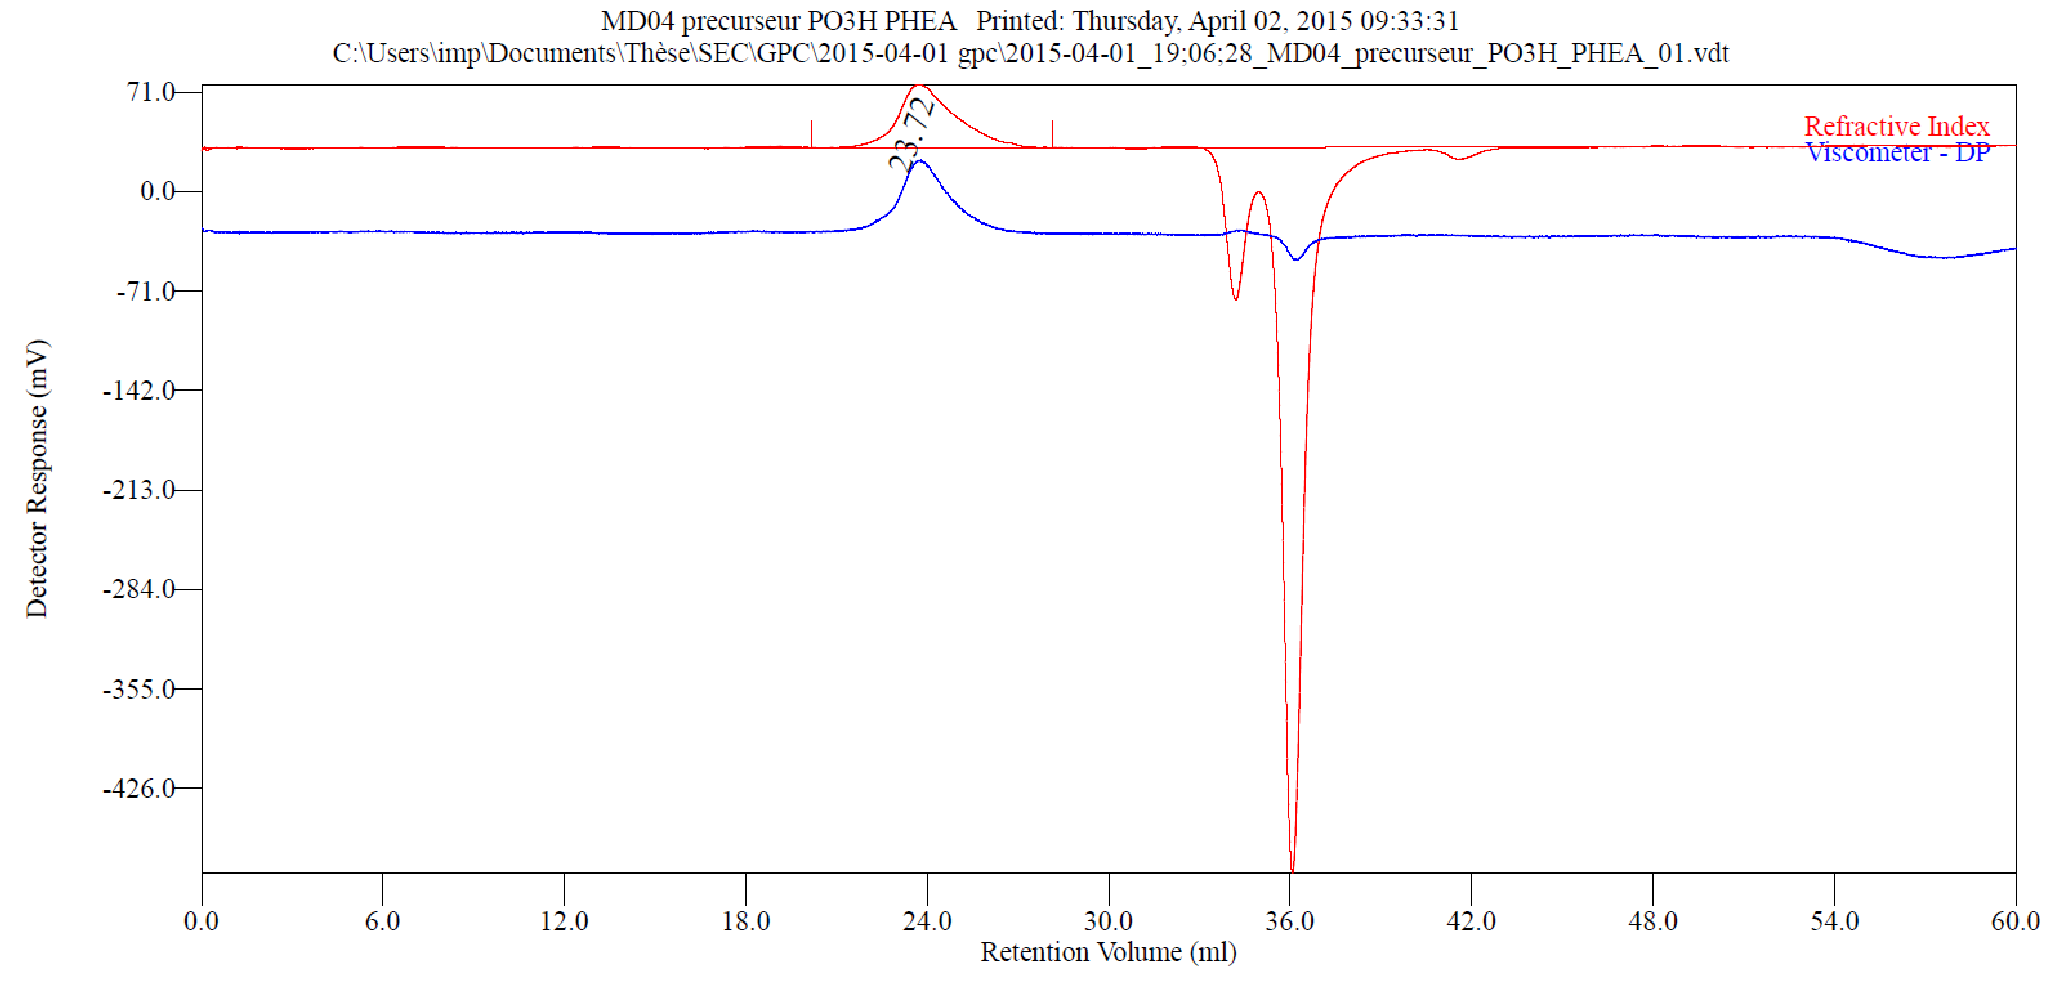
\includegraphics[width=\textwidth]{sec_spectra.png}
\begin{tabular}{llll}
Peak RV - (ml) & 23.72 & 
Mn - (Daltons) & 5 155 \\
Mw - (Daltons) & 5 614 &
Mz - (Daltons) & 5 985 \\
Mp - (Daltons) & 7 221 &
Mw / Mn & 1.089\\
Percent Above Mw: 0 & 100.0 &
Percent Below Mw: 0 & 0.0\\
Mw 10.0\% Low & 3 012 &
Mw 10.0\% High & 7 087\\
IV - (dl/g) & 0.6026 &
Rh(w) - (nm) & 3.899\\
Wt Fr (Peak) & 1.000 &\\
Mark-Houwink a & 0.331&
Mark-Houwink logK & -1.453\\
Branches & 0.000 &
Branch Freq. & 0.000\\
RI Area - (mvml) & 98.76 &
UV Area - (mvml) & 0.00\\
RALS Area - (mvml) & 0.00 &
LALS Area - (mvml) & 0.00\\
IVDP Area - (mvml) & 105.24\\
\end{tabular}
\caption{SEC Spectra of \ce{POH}.}
\label{fig:sec}
\end{figure}

\begin{figure}
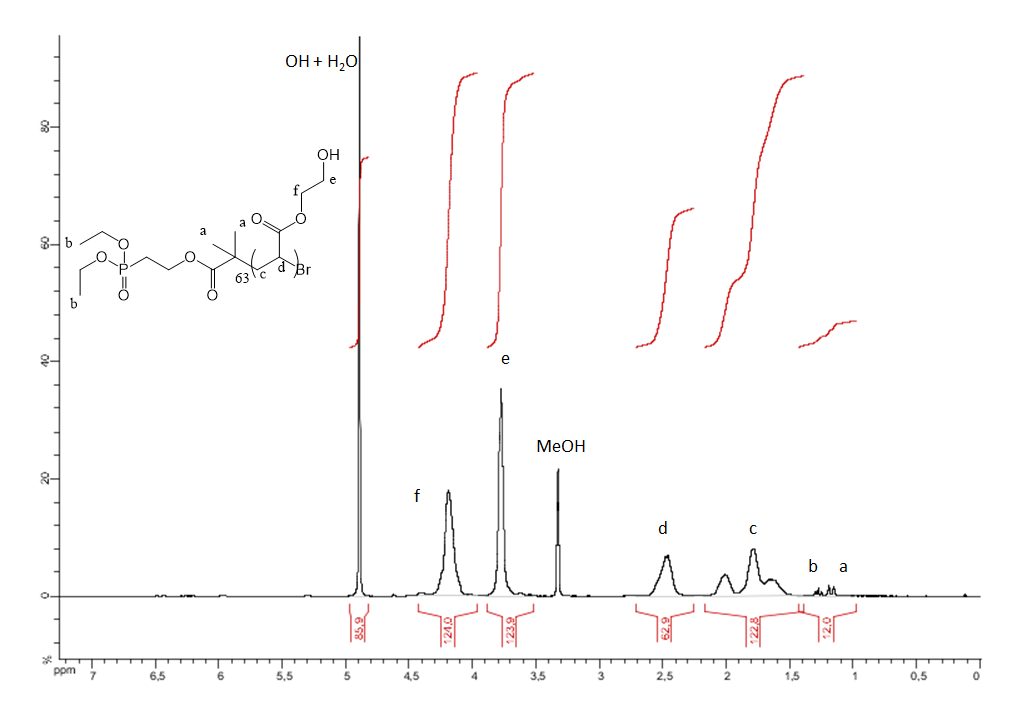
\includegraphics[width=\textwidth]{POH_1H_NMR.png}
\caption{1H NMR of POH in deuterated methanol, with signal attribution. Calibration of the integrals intensity, relative to the distinct chain-end signals (a and b, 6 protons each), allows us to determine polymer chain length $n$ (here, considering integration of signal d,  $n=69-70$, $Mn=\SI{8335}{\dalton}$)}
\end{figure}

\begin{figure}
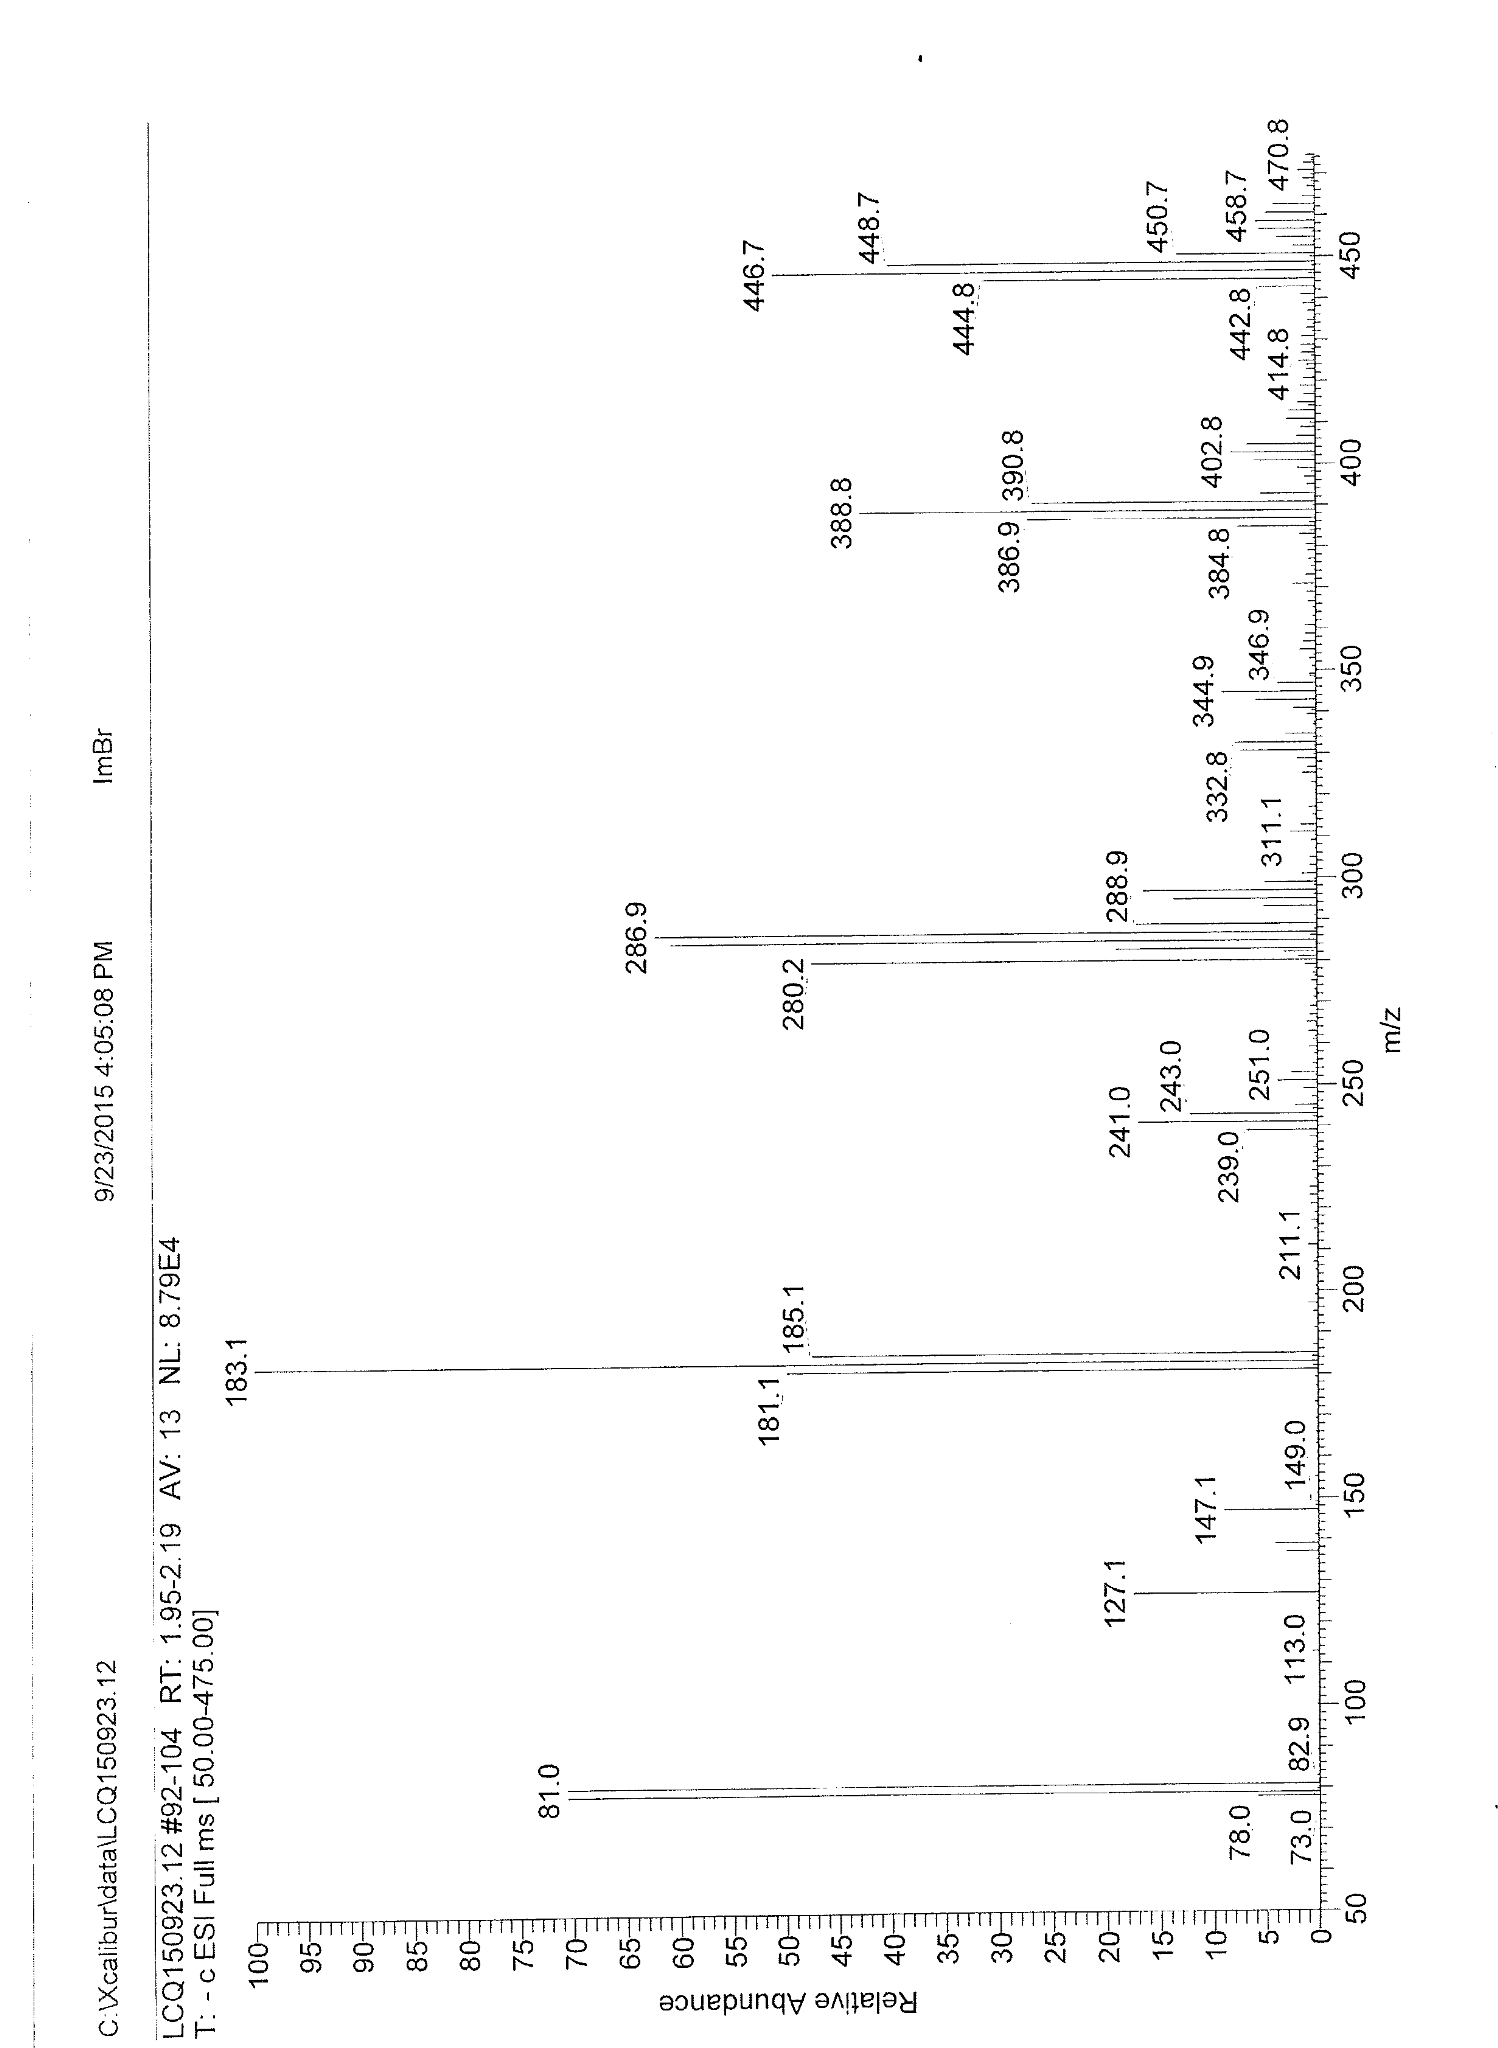
\includegraphics[height=\textheight-2\baselineskip]{mass_PImBr.png}
\caption{High resolution mass spectra of \ce{PIm+Br-}. Bromide peak exist at m/z=81.0.}
\label{fig:massPImBr}
\end{figure}

\begin{figure}
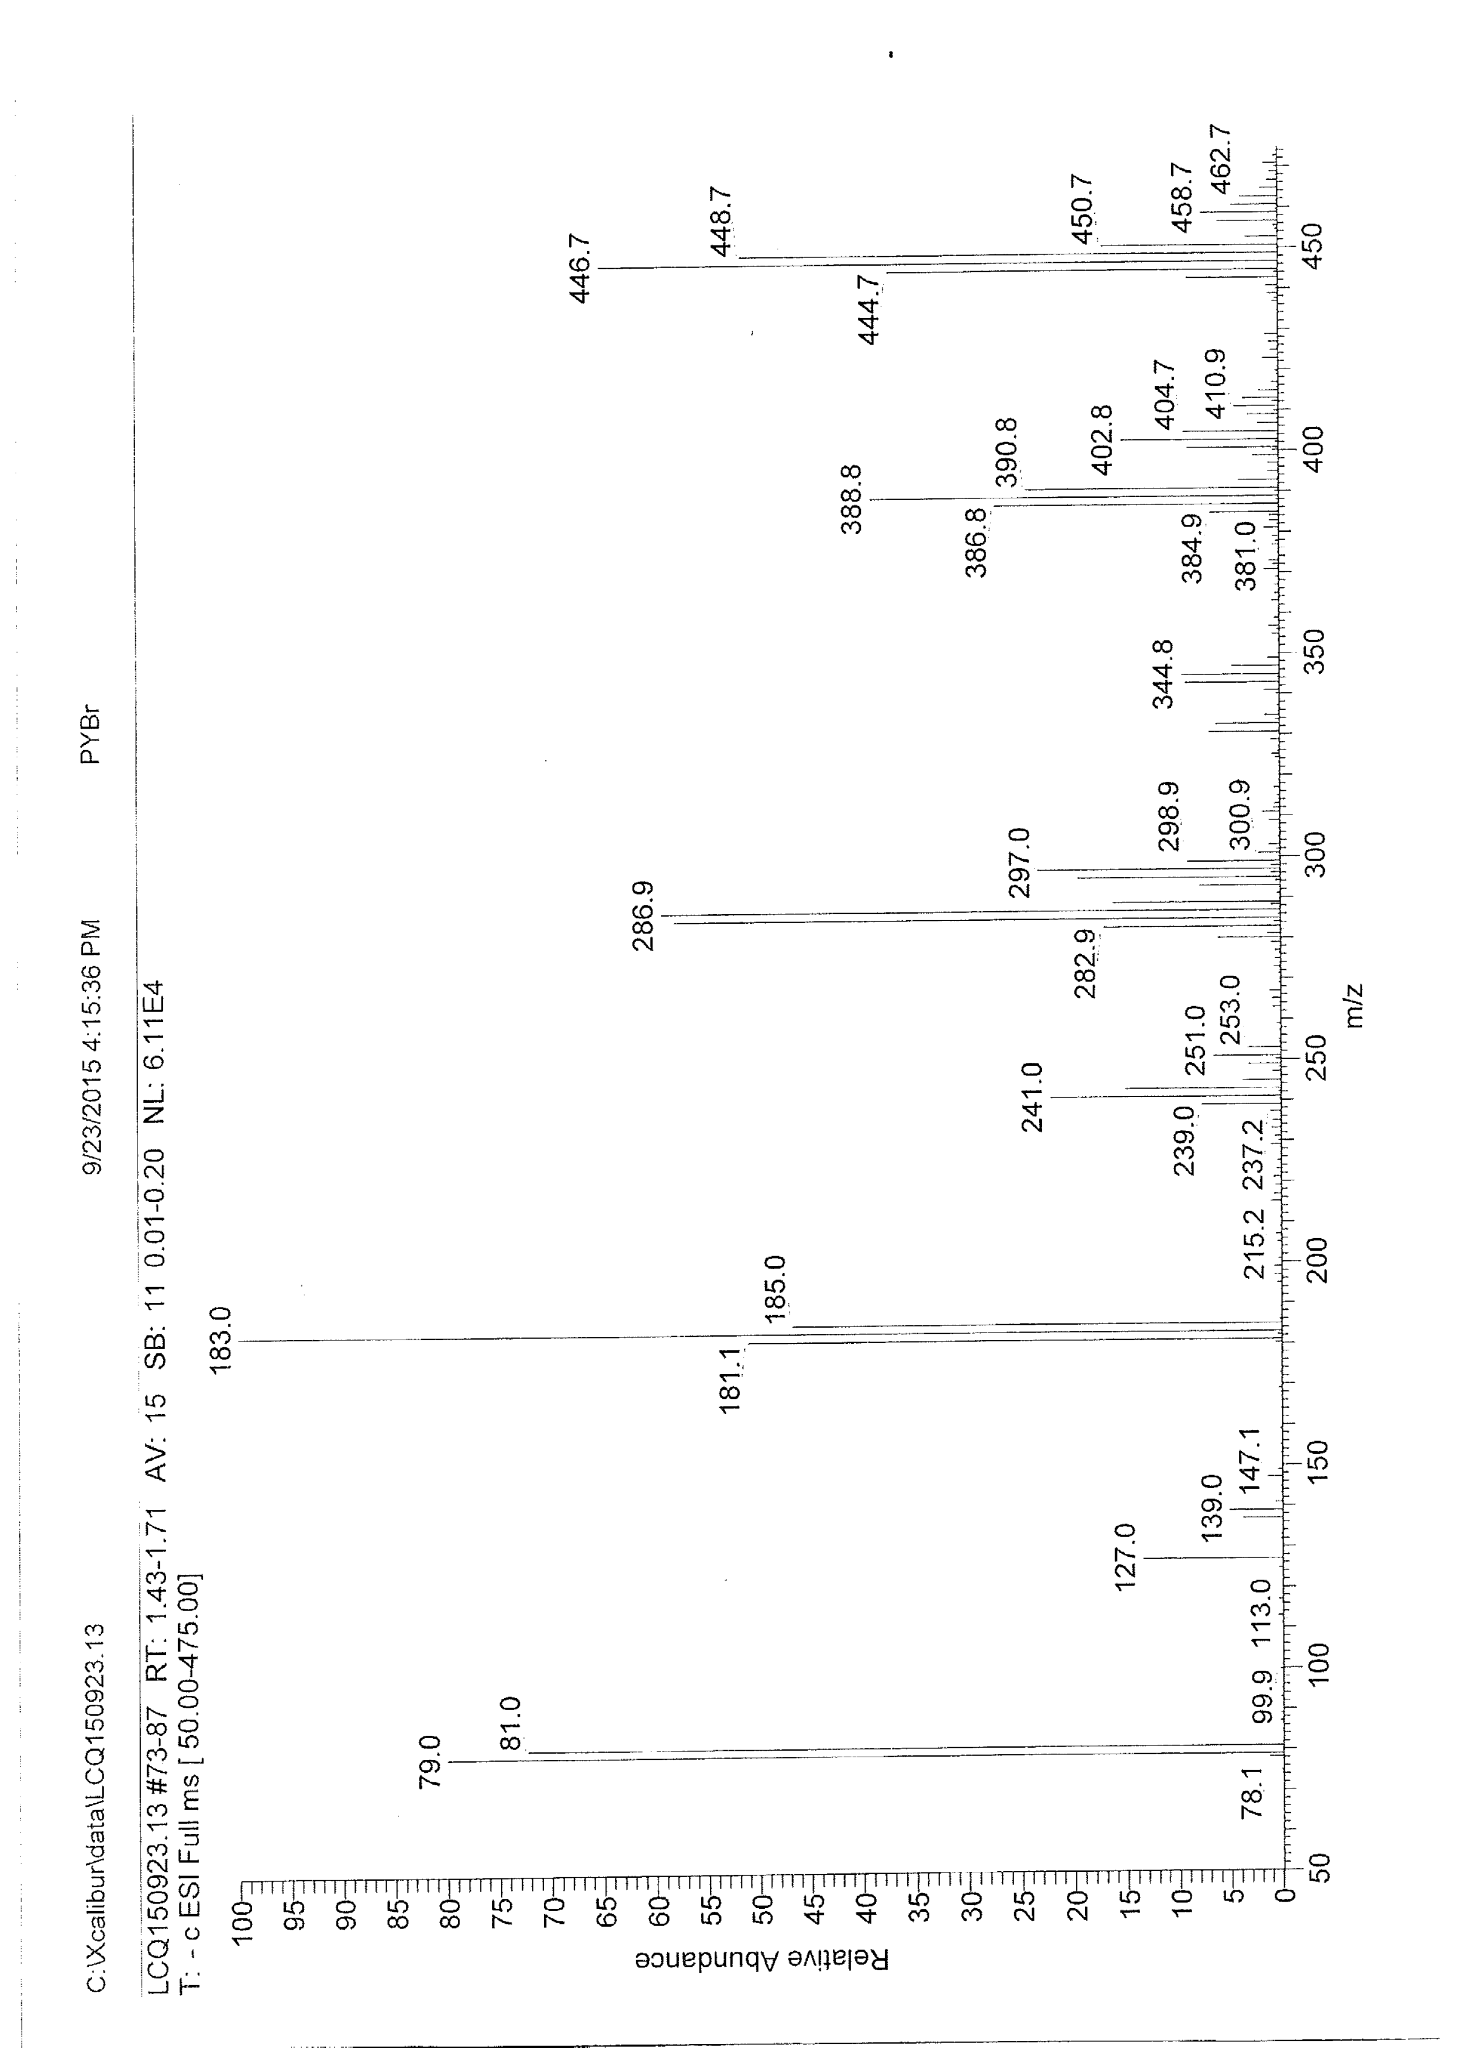
\includegraphics[height=\textheight-2\baselineskip]{mass_PPyBr.png}
\caption{High resolution mass spectra of \ce{PPy+Br-}. Bromide peak exist at m/z=79-81.}
\label{fig:massPPyBr}
\end{figure}

\begin{figure}
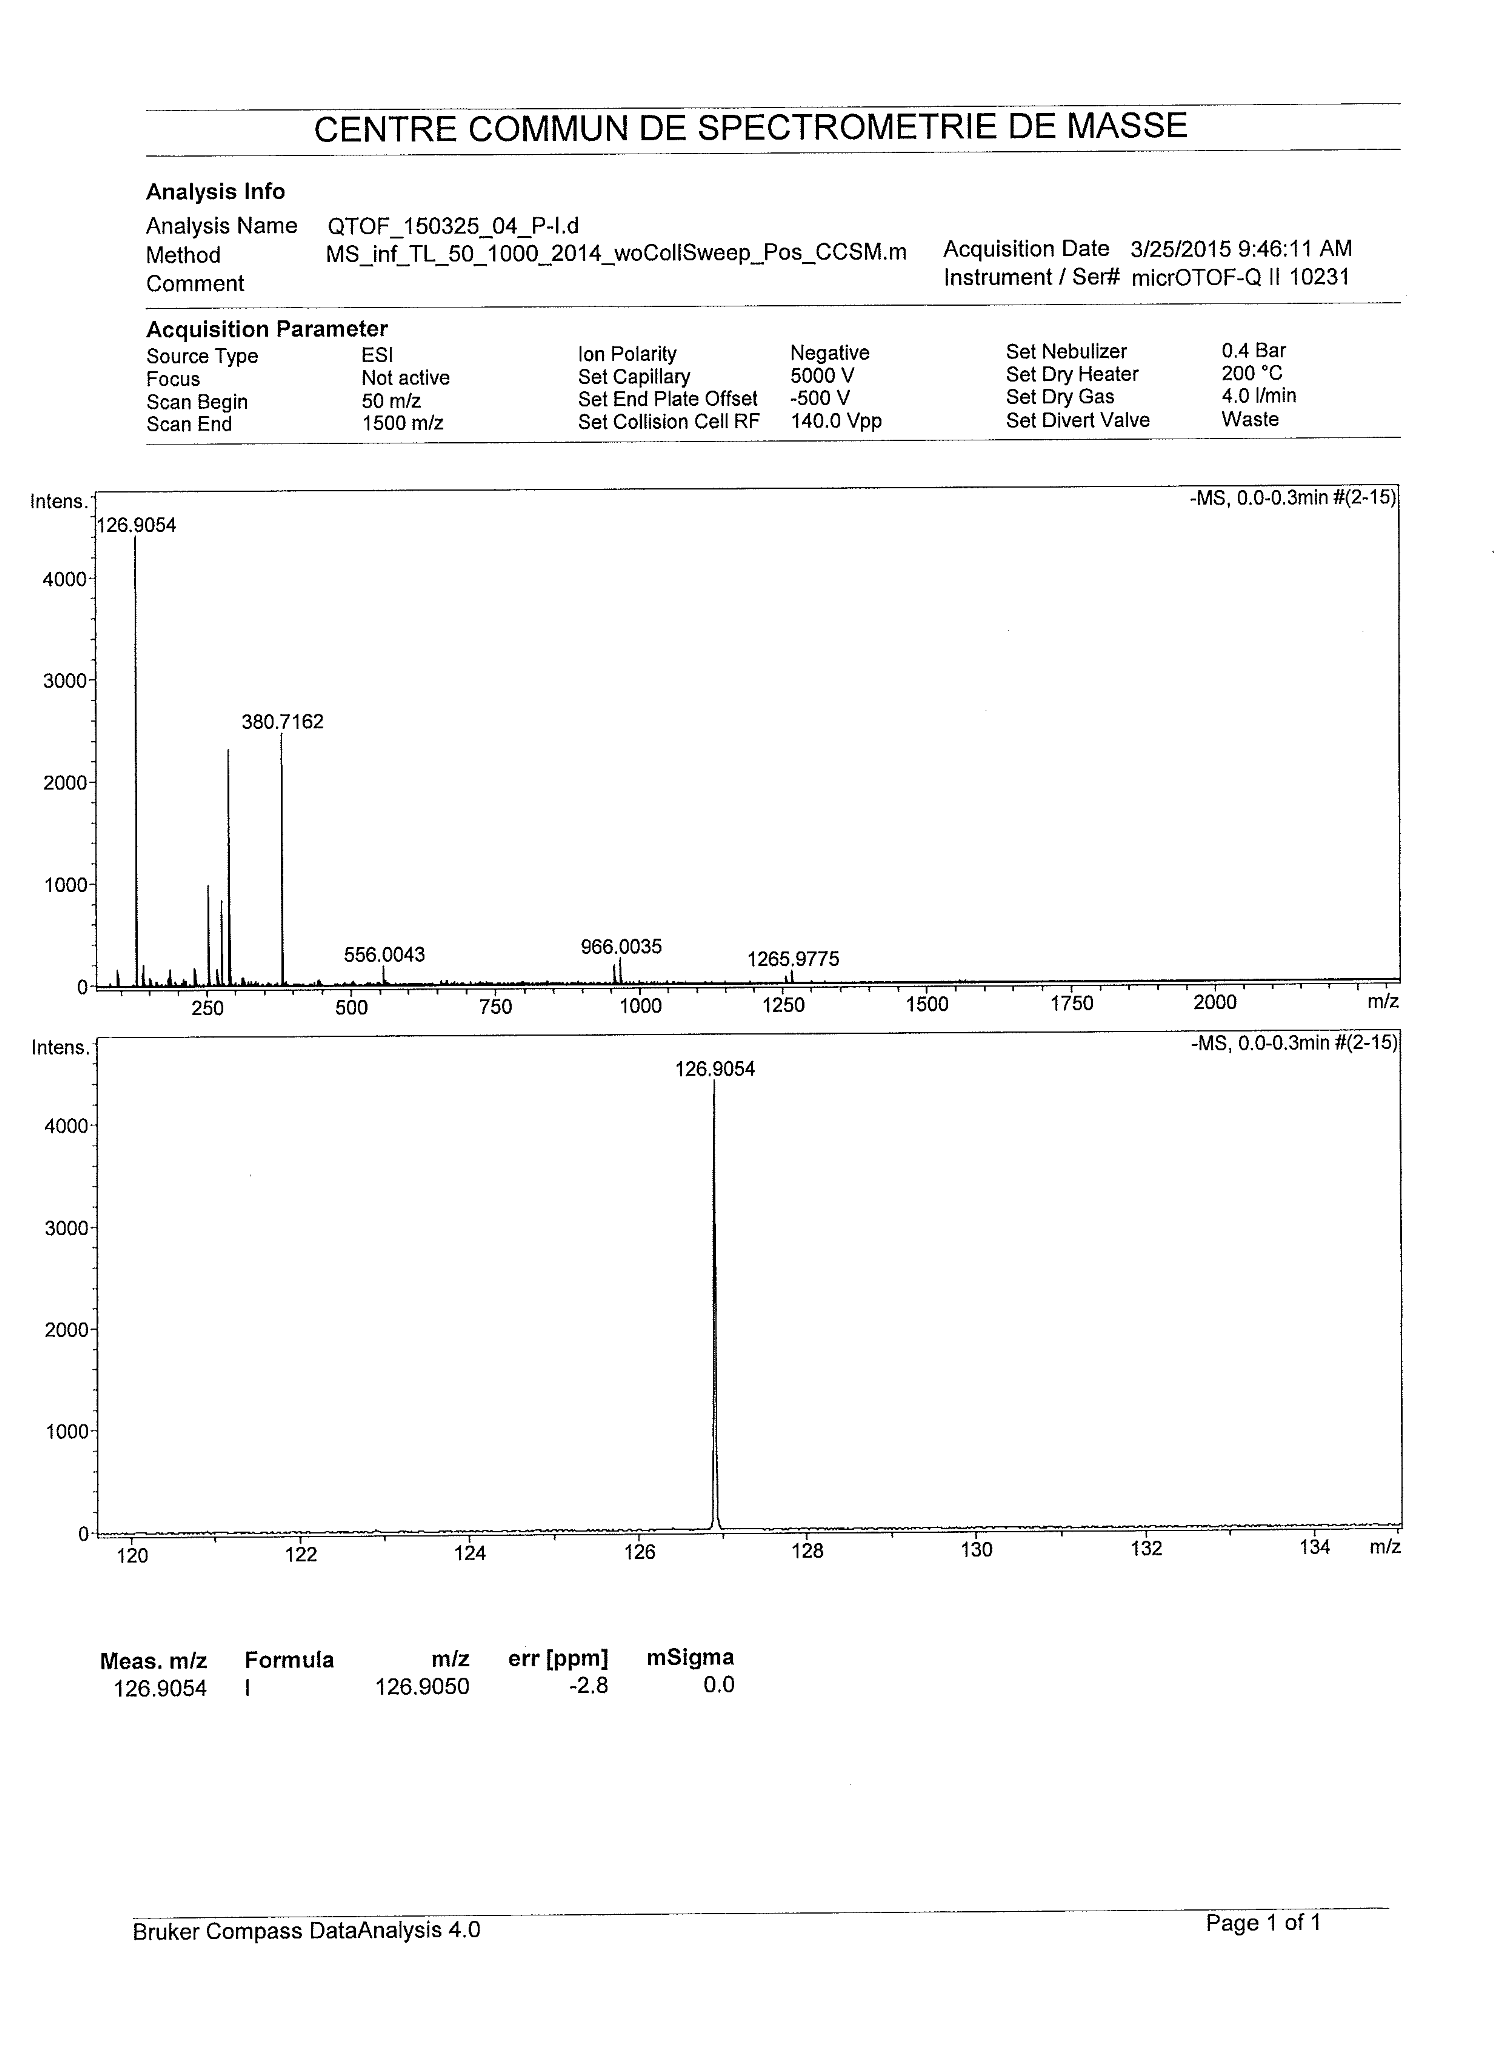
\includegraphics[height=\textheight-2\baselineskip]{mass_PImI.png}
\caption{High resolution mass spectra of \ce{PIm+I-}. Iodide peak exist at m/z=126.9.}
\label{fig:massPImI}
\end{figure}

\begin{figure}
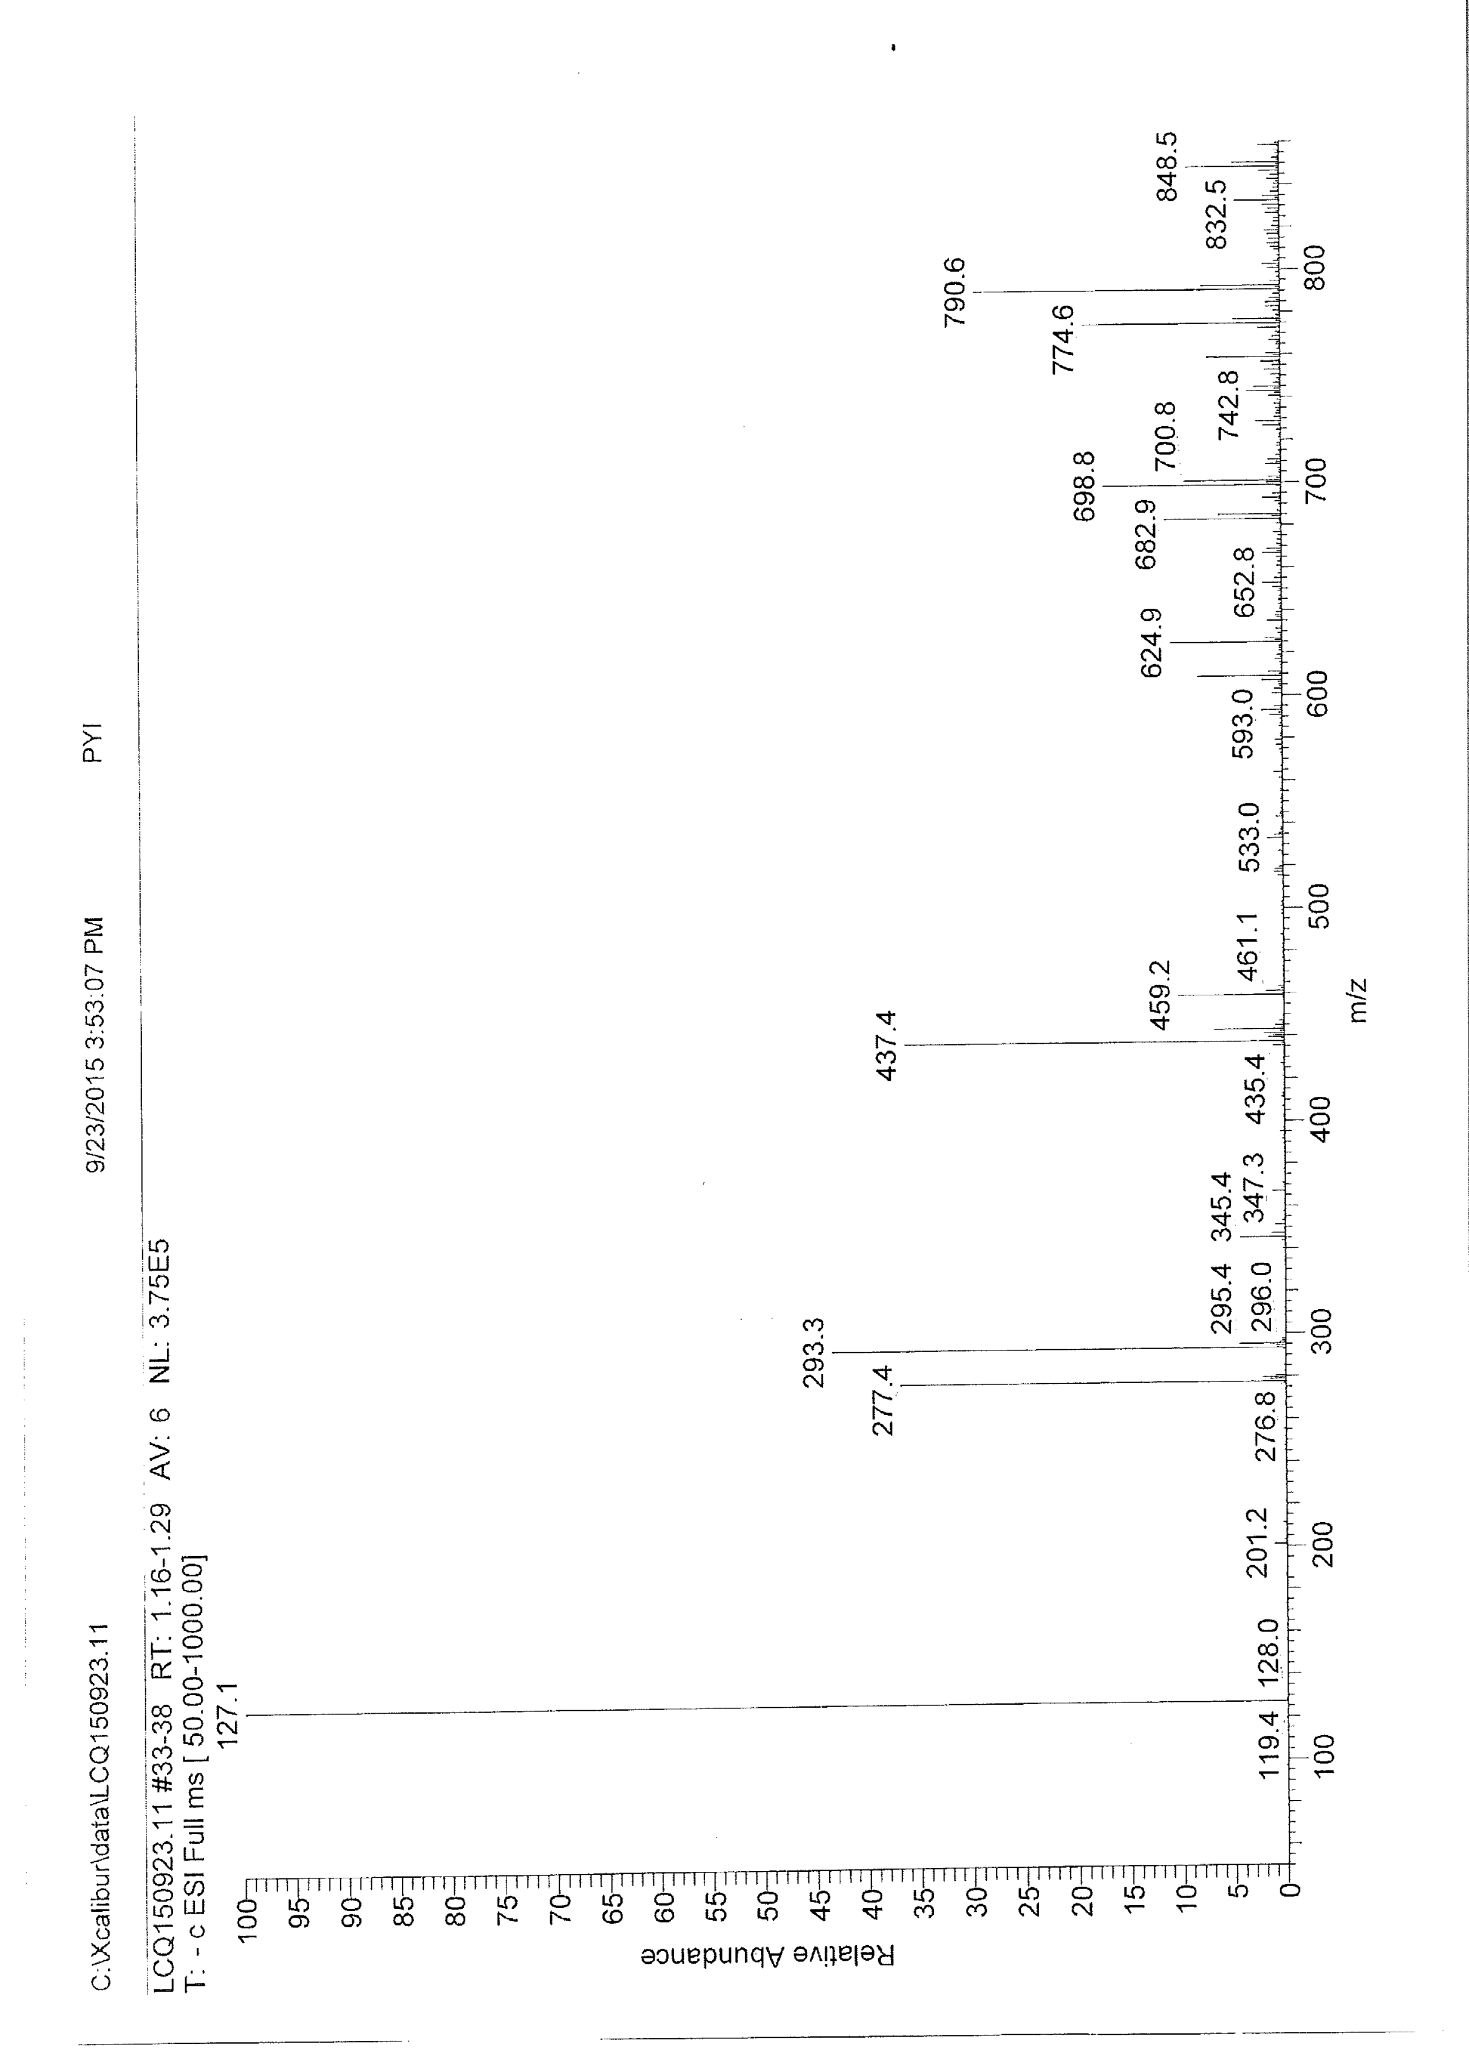
\includegraphics[height=\textheight-2\baselineskip]{mass_PPyI.png}
\caption{High resolution mass spectra of \ce{PPy+I-}. Iodide peak exist at m/z=127.1.}
\label{fig:massPPyI}
\end{figure}

\begin{figure}
\includegraphics{frequency.pdf}
\caption{Storage modulus $G^\prime$ ($\bullet$) and loss modulus $G^{\prime\prime}$ ($\square$) measured through oscillatory shear experiments plotted against the frequency $f$. The moieties change with rows and the counterions with columns. The fixed strain amplitude is $\gamma=0.1\%$. All samples are at 7.4~wt\%. }
\label{fig:frequency}
\end{figure}

\end{document}